% Slides: computing on several devices (CPUs, GPUs, and Apple's MPS) from
% torch, for an informal talk to graduate students on 2026-09-25.
% Same look as the mbirtorch update deck in ../mbirtorch_update_2026-09.
% Build: latexmk devices_talk_deck.tex (see latexmkrc).
% Figures: run the demos in demos/, then make_figures.py; README.md names the
% source of every image and number.
%
% A frame body must not start with a brace group: beamer would read it as the
% frame's subtitle, which this theme does not show.  Start with \vspace{0pt}.
\documentclass[aspectratio=169,10pt]{beamer}
\usepackage[T1]{fontenc}
\usepackage[utf8]{inputenc}
\usetheme[progressbar=frametitle,numbering=fraction]{metropolis}
\usepackage[sfdefault,lining]{FiraSans}
\usepackage{FiraMono}
\usepackage{amsmath}
\usepackage{graphicx}
\usepackage{array}
\usepackage{colortbl}
\usepackage{calc}
\usepackage{listings}
\usepackage{appendixnumberbeamer}
\usepackage{tikz}
\usetikzlibrary{positioning,arrows.meta,calc}
\graphicspath{{images/}{../mbirtorch_update_2026-09/images/}}

\definecolor{planAccent}{HTML}{3D6B99}   % device memory, measured values
\definecolor{safeGreen}{HTML}{2E7D32}    % NVLink, compute-bound work
\definecolor{axialBrick}{HTML}{A23B3B}   % PCIe, host waits, exchanges
\definecolor{branchAmber}{HTML}{B26B1F}
\definecolor{inkGray}{HTML}{5A5A5A}
\definecolor{barGray}{HTML}{262626}

\setbeamercolor{frametitle}{bg=barGray, fg=white}

\newcommand{\speclabel}[1]{\textcolor{inkGray}{\scriptsize\MakeUppercase{#1}}}

% A note with the accent bar; the bar spans the whole note.
\newsavebox{\notebox}
\newcommand{\noteline}[1]{%
  \savebox{\notebox}{\begin{minipage}[b]{0.94\linewidth}\raggedright
    {\small\textcolor{inkGray}{#1}}\end{minipage}}%
  {\color{planAccent}\rule[-\dp\notebox]{2pt}{\dimexpr\ht\notebox+\dp\notebox\relax}}%
  \hspace{6pt}\usebox{\notebox}}

% The same note bar in footnotesize, for a slide that is short of room.
\newcommand{\footnoteline}[1]{%
  \savebox{\notebox}{\begin{minipage}[b]{0.94\linewidth}\raggedright
    {\footnotesize\textcolor{inkGray}{#1}}\end{minipage}}%
  {\color{planAccent}\rule[-\dp\notebox]{2pt}{\dimexpr\ht\notebox+\dp\notebox\relax}}%
  \hspace{6pt}\usebox{\notebox}}

% A record cited at the foot of a slide.
\newcommand{\source}[1]{\par\vfill{\scriptsize\textcolor{inkGray}{Source: #1}\par}}

% A light rule between the rows of a table whose cells wrap.
\newcommand{\rowrule}{\\[3pt]\arrayrulecolor{inkGray!35}\hline\noalign{\vskip 3pt}}

% A caption under a figure.
\newcommand{\figcaption}[1]{{\scriptsize\textcolor{inkGray}{#1}\par}}

\newcommand{\head}[1]{\textbf{#1}}

% Code on a slide.  A frame that holds a listing must be [fragile].
\lstset{language=Python, basicstyle=\ttfamily\scriptsize, keywordstyle=\color{planAccent}\bfseries,
  commentstyle=\color{inkGray}, stringstyle=\color{safeGreen}, columns=fullflexible,
  keepspaces=true, showstringspaces=false, aboveskip=3pt, belowskip=3pt}

\title{Computing on several devices}
\subtitle{CPUs, GPUs, and Apple's MPS in torch, with examples from mbirtorch}
\author{Greg Buzzard}
\date{September 25, 2026}

\begin{document}

\maketitle

% ================================================================ overview
\begin{frame}{What this talk covers}
  \medskip
  {\large A computer is a set of processors and memories joined by links.
  The links differ in speed by a factor of 50 or more.  Most of the work of
  making code fast is keeping data near the processor that uses it, and
  keeping every processor busy.}\par\vspace{6pt}
  {\small
  \begin{columns}[T]
    \begin{column}{0.50\textwidth}
      \begin{enumerate}
        \item The devices: CPUs, GPUs, MPS, and the links between them.
        \item Where the time goes: four limits on speed.
        \item Threads: three meanings of one word.
        \item One device, fully used: batching, compiling, and hand-written kernels.
      \end{enumerate}
    \end{column}
    \begin{column}{0.48\textwidth}
      \begin{enumerate}\setcounter{enumi}{4}
        \item Several devices: independent jobs, sharding, and splitting a problem.
        \item Memory: where it goes, and what a copy costs.
        \item Measuring honestly.
      \end{enumerate}
    \end{column}
  \end{columns}\vspace{4pt}
  The measured numbers come from mbirtorch records and from five short demos
  run on an M4 Max laptop.  The demo scripts are in \texttt{demos/} beside
  these slides, and each one runs without change on a CUDA GPU.}
\end{frame}

% ================================================================ 1 DEVICES
\section{The devices}

% ---------------------------------------------------------------- kinds
\begin{frame}{Three kinds of device}
  \begin{columns}[T]
    \begin{column}{0.44\textwidth}
      {\small
      \head{CPU.}  A CPU has up to about a hundred general-purpose cores with
      large caches.  It works in host memory, the main memory of the
      computer.  In torch it is \texttt{'cpu'}.\par\vspace{5pt}
      \head{GPU.}  A GPU has thousands of simple arithmetic units that apply
      one instruction to many values at once.  It has its own memory, and it
      reaches host memory over the PCIe bus.  In torch it is \texttt{'cuda:0'},
      \texttt{'cuda:1'}, and so on.\par\vspace{5pt}
      \head{MPS.}  MPS is torch's back end for the GPU in Apple silicon.  That
      GPU shares one memory with the CPU.  In torch it is \texttt{'mps'}.  MPS
      has no float64.\par}
    \end{column}
    \begin{column}{0.54\textwidth}
      {\footnotesize
      \begin{tabular}{@{}>{\raggedright\arraybackslash}p{0.20\linewidth}@{\hspace{5pt}}>{\raggedright\arraybackslash}p{0.37\linewidth}@{\hspace{5pt}}>{\raggedright\arraybackslash}p{0.36\linewidth}@{}}
        & \speclabel{m4 max laptop} & \speclabel{one gautschi node} \rowrule
        cores & 12 + 4 CPU cores, and a GPU with 40 cores & 112 CPU cores, and 8 H100 GPUs \rowrule
        memory & 128 GB, shared & 1 TB on the host, and 80 GB on each GPU \rowrule
        memory bandwidth & 546 GB/s, shared (432 GB/s measured on the GPU) & 3.35 TB/s from each GPU's 80 GB \rowrule
        host to GPU & no separate link (a copy measured 89 GB/s) & PCIe 5, 64 GB/s each way \rowrule
        GPU to GPU & none & NVLink, 900 GB/s \rowrule
        float32 & 13.4 TFLOP/s measured on the GPU & 67 TFLOP/s on each GPU \\
      \end{tabular}}
    \end{column}
  \end{columns}
  \source{Apple M4 Max and NVIDIA H100 SXM specifications; \texttt{.claude/cluster\_use.md};
  \texttt{demos/demo\_machine.py}}
\end{frame}

% ---------------------------------------------------------------- links
\begin{frame}{The links differ in speed by a factor of 50}
  \centering
  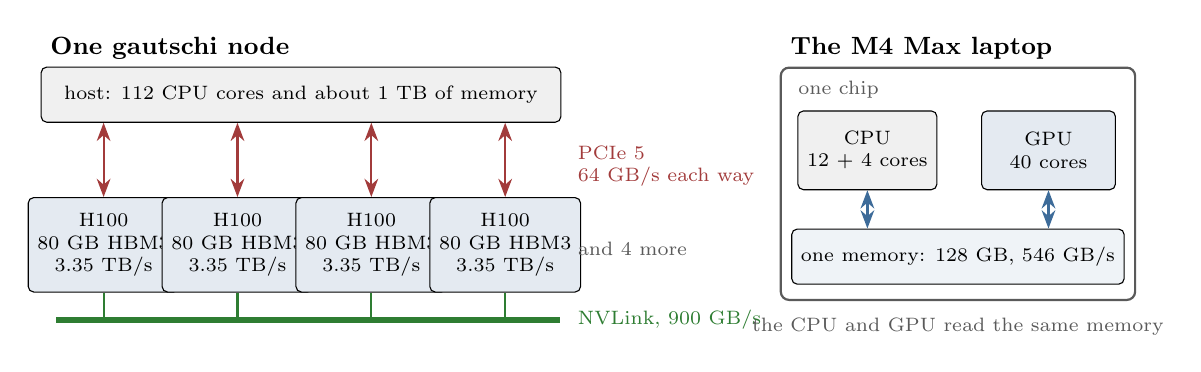
\begin{tikzpicture}[>=Stealth, font=\scriptsize,
      host/.style={draw, rounded corners=2pt, fill=gray!12, align=center},
      gpu/.style={draw, rounded corners=2pt, fill=planAccent!14, minimum width=14mm, minimum height=10mm, align=center},
      hbm/.style={gpu, minimum height=12mm},
      pcie/.style={<->, thick, axialBrick},
      own/.style={<->, thick, planAccent}]
    % ---- one gautschi node
    \node[font=\small\bfseries, anchor=west] at (0,3.75) {One gautschi node};
    \node[host, anchor=south west, minimum width=66mm, minimum height=7mm] (host) at (0,2.8)
      {host: 112 CPU cores and about 1 TB of memory};
    \foreach \i in {0,1,2,3} {
      \node[hbm] (g\i) at (0.8+1.7*\i, 1.25) {H100\\80 GB HBM3\\3.35 TB/s};
      \draw[pcie] (g\i.north |- host.south) -- (g\i.north);
    }
    \node[anchor=west, text=inkGray] at (6.7,1.2) {and 4 more};
    \node[axialBrick, anchor=west, align=left] at (6.7,2.25) {PCIe 5\\64 GB/s each way};
    \draw[safeGreen, line width=2.2pt] (0.2,0.3) -- (6.6,0.3);
    \foreach \i in {0,1,2,3} { \draw[safeGreen, thick] (g\i.south) -- (g\i.south |- 0,0.3); }
    \node[safeGreen, anchor=west] at (6.7,0.3) {NVLink, 900 GB/s};
    % ---- the M4 Max
    \begin{scope}[xshift=94mm]
      \node[font=\small\bfseries, anchor=west] at (0,3.75) {The M4 Max laptop};
      \draw[rounded corners=3pt, thick, draw=inkGray] (0,0.55) rectangle (4.5,3.5);
      \node[anchor=north west, text=inkGray] at (0.1,3.45) {one chip};
      \node[host, minimum width=17mm, minimum height=10mm] (cpu) at (1.1,2.45) {CPU\\12 + 4 cores};
      \node[gpu, minimum width=17mm] (mgpu) at (3.4,2.45) {GPU\\40 cores};
      \node[host, fill=planAccent!8, minimum width=40mm, minimum height=7mm] (mem) at (2.25,1.1)
        {one memory: 128 GB, 546 GB/s};
      \draw[own] (cpu.south) -- (cpu.south |- mem.north);
      \draw[own] (mgpu.south) -- (mgpu.south |- mem.north);
      \node[anchor=north, text=inkGray] at (2.25,0.45) {the CPU and GPU read the same memory};
    \end{scope}
  \end{tikzpicture}\par\vspace{4pt}
  \noteline{PCIe brings data from host memory to an H100 at 64 GB/s at most.
  In the time one array arrives, the H100 can read about 50 arrays of the same
  size from its own memory.  On the M4 Max the same ratio is about 5, from the
  measured rates of 432 GB/s and 89 GB/s.  The copy itself is faster on the Mac
  than on gautschi.  It is a smaller share of the time because the Mac's GPU
  memory is slower.  A loop that copies data in every step can therefore spend
  most of its time copying on gautschi, even when it runs well on the Mac.}
  \source{NVIDIA H100 SXM and Apple M4 Max specifications; \texttt{demos/demo\_machine.py}}
\end{frame}

% ================================================================ 2 LIMITS
\section{Where the time goes}

% ---------------------------------------------------------------- four limits
\begin{frame}{Four limits on speed}
  \vspace{0pt}
  {\small Every operation is limited by one of four things, and the remedy
  depends on which one.}\par\vspace{6pt}
  {\footnotesize
  \begin{tabular}{@{}>{\raggedright\arraybackslash}p{0.14\linewidth}@{\hspace{6pt}}>{\raggedright\arraybackslash}p{0.30\linewidth}@{\hspace{6pt}}>{\raggedright\arraybackslash}p{0.24\linewidth}@{\hspace{6pt}}>{\raggedright\arraybackslash}p{0.26\linewidth}@{}}
    \speclabel{limit} & \speclabel{what sets it} & \speclabel{where it appears} & \speclabel{what helps} \rowrule
    \head{Overhead} & the host's cost to issue each operation, 3 microseconds on the M4 Max GPU, or 140 if the host waits for each result & many small operations, and loops that read values back to the host & batching, compiling, and no host waits inside loops \rowrule
    \head{Memory bandwidth} & the rate at which data moves between memory and the processor, or over PCIe for a copy & elementwise operations, gathers, and scatters, as in back projection & fewer bytes moved: fused operations, fewer temporary arrays, smaller types \rowrule
    \head{Compute} & the rate of arithmetic & large matrix products and convolutions & tensor cores (TF32, bfloat16), where their precision is enough \rowrule
    \head{Capacity} & the size of the memory & out-of-memory errors & sharding, splitting, or streaming (Section 5) \\
  \end{tabular}}
  \source{\texttt{demos/demo\_machine.py} and \texttt{demos/demo\_sizes.py}}
\end{frame}

% ---------------------------------------------------------------- intensity
\begin{frame}{Arithmetic intensity decides between bandwidth and compute}
  \begin{columns}[T]
    \begin{column}{0.46\textwidth}
      {\small
      \head{Arithmetic intensity} is the number of arithmetic operations per
      byte moved to or from memory.  A device's \head{balance point} is its
      arithmetic rate divided by its memory bandwidth.  It is 20 operations
      per byte for an H100, and 31 for the M4 Max GPU.  Work below the
      balance point is limited by bandwidth, and work above it by
      arithmetic.\par\vspace{5pt}
      Adding two float32 arrays has intensity 1/12.  A product of two
      $n \times n$ matrices has intensity $n/6$.\par\vspace{5pt}
      Projectors have low intensity.  Moving fewer bytes speeds them up, and
      faster arithmetic does not.\par}
    \end{column}
    \begin{column}{0.52\textwidth}
      \centering
      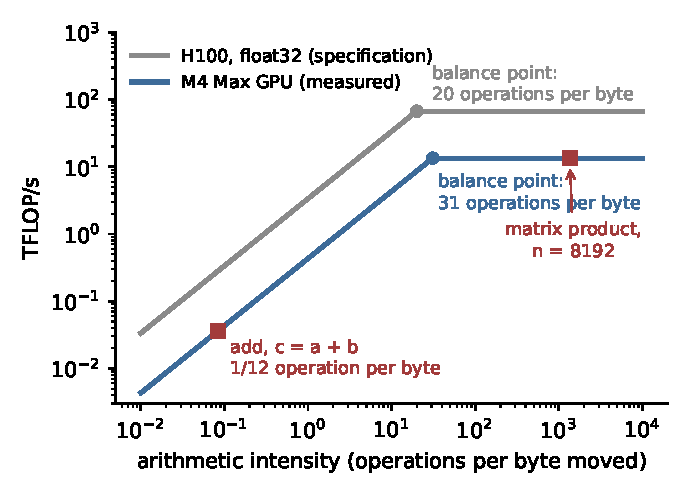
\includegraphics[width=\linewidth]{roofline.pdf}\\[2pt]
      \figcaption{Each line is the highest rate a device can reach at a given
      intensity.  The squares are the add and the matrix product measured on
      the M4 Max GPU.}
    \end{column}
  \end{columns}
  \source{\texttt{demos/demo\_machine.py}; NVIDIA H100 SXM specification}
\end{frame}

% ---------------------------------------------------------------- threads scaling
\begin{frame}{Compute-bound work scales with cores, and bandwidth-bound work does not}
  \begin{columns}[T]
    \begin{column}{0.46\textwidth}
      {\small
      The demo times two operations on arrays of $2^{26}$ float32 values, far
      more than the caches hold.\par\vspace{5pt}
      \head{sin} does many operations per byte.  It ran about 9 times faster
      on 12 threads than on one.\par\vspace{5pt}
      \head{add} does 1 operation per 12 bytes.  It stopped gaining at 4
      threads, because the cores had reached the memory
      bandwidth.\par\vspace{5pt}
      The 4 efficiency cores slowed sin down, because each thread gets an
      equal part of the array.\par\vspace{6pt}}
      \footnoteline{mbirjax saw the same pattern on CPU devices.  The
      compute-bound filter ran 5 to 6 times faster, and back projection only
      1.5 times.}
    \end{column}
    \begin{column}{0.52\textwidth}
      \centering
      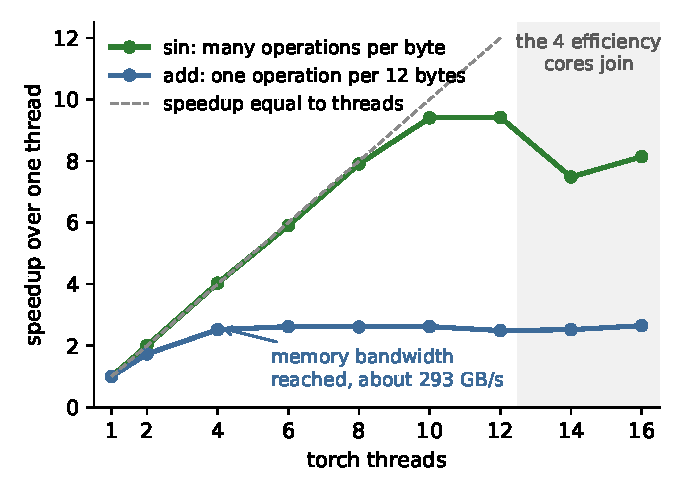
\includegraphics[width=\linewidth]{thread_scaling.pdf}\\[2pt]
      \figcaption{Speedup over one thread on the M4 Max CPU, for arrays of
      $2^{26}$ float32 values.}
    \end{column}
  \end{columns}
  \source{\texttt{demos/demo\_threads.py}; \texttt{.claude/lessons.md}, Section 6}
\end{frame}

% ================================================================ 3 THREADS
\section{Threads}

% ---------------------------------------------------------------- three meanings
\begin{frame}{One word, three meanings}
  \vspace{0pt}
  {\footnotesize
  \begin{tabular}{@{}>{\raggedright\arraybackslash}p{0.16\linewidth}@{\hspace{6pt}}>{\raggedright\arraybackslash}p{0.30\linewidth}@{\hspace{6pt}}>{\raggedright\arraybackslash}p{0.18\linewidth}@{\hspace{6pt}}>{\raggedright\arraybackslash}p{0.28\linewidth}@{}}
    & \speclabel{what it is} & \speclabel{how many} & \speclabel{set by} \rowrule
    \head{torch's CPU threads} & a pool that splits one CPU operation across cores & about one per core & \texttt{OMP\_NUM\_THREADS} or \texttt{torch.set\_num\_threads} \rowrule
    \head{Host threads} & Python threads, each issuing work to one device & one per device & your code, with \texttt{threading} or \texttt{ThreadPoolExecutor} \rowrule
    \head{GPU threads} & lightweight threads inside one GPU kernel, run in groups of 32 & thousands to millions in one kernel & the author of the kernel, in Triton or CUDA \\
  \end{tabular}}\par\vspace{10pt}
  \noteline{Ordinary torch code meets only the first two kinds.  The first kind
  makes one CPU operation faster.  The second kind keeps several devices busy at
  once.  The third kind matters only to someone who writes a kernel.}
\end{frame}

% ---------------------------------------------------------------- async
\begin{frame}[fragile]{A GPU call returns before the GPU finishes}
  \begin{columns}[T]
    \begin{column}{0.48\textwidth}
      {\small
      torch puts each GPU operation in a queue, called a stream, and returns
      at once.  The GPU runs the queue in order while the host goes on.  The
      host waits only when it needs a value.\par\vspace{5pt}
      {\footnotesize
      \begin{tabular}{@{}l@{\hspace{16pt}}r@{}}
        \speclabel{an 8192 by 8192 matrix product on mps} & \speclabel{time} \\[2pt]
        the call returned & 0.11 ms \\
        \texttt{synchronize()} returned & 81.9 ms \\
        \texttt{.item()} returned & 82.0 ms \\
      \end{tabular}}\par\vspace{5pt}
      A timing without \texttt{synchronize()} measures only the launch.  Any
      call that brings a value to the host waits for the queue to empty:
      \texttt{.item()}, \texttt{float(t)}, \texttt{.cpu()},
      \texttt{print(t)}, and \texttt{if t > 0}.  In a loop, each such wait
      leaves the GPU idle.\par}
    \end{column}
    \begin{column}{0.50\textwidth}
      \centering
      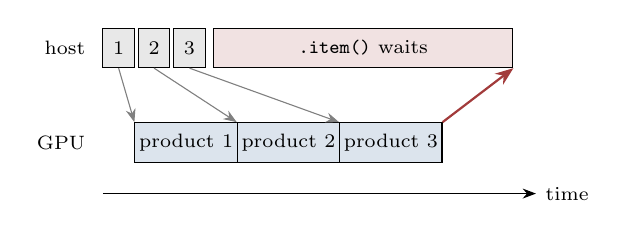
\begin{tikzpicture}[font=\scriptsize, >=Stealth,
          op/.style={draw, fill=planAccent!18, minimum height=5mm, inner sep=1pt},
          launch/.style={draw, fill=gray!18, minimum height=5mm, minimum width=4mm, inner sep=1pt}]
        \node[anchor=east] at (-0.1,1.6) {host};
        \node[anchor=east] at (-0.1,0.4) {GPU};
        \node[launch] (l1) at (0.2,1.6) {1};
        \node[launch] (l2) at (0.65,1.6) {2};
        \node[launch] (l3) at (1.1,1.6) {3};
        \node[draw, fill=axialBrick!15, minimum height=5mm, minimum width=38mm, anchor=west] (w) at (1.4,1.6) {\texttt{.item()} waits};
        \node[op, minimum width=13mm, anchor=west] (k1) at (0.4,0.4) {product 1};
        \node[op, minimum width=13mm, anchor=west] (k2) at (1.7,0.4) {product 2};
        \node[op, minimum width=13mm, anchor=west] (k3) at (3.0,0.4) {product 3};
        \foreach \a/\b in {l1/k1, l2/k2, l3/k3} { \draw[->, gray] (\a.south) -- (\b.north west); }
        \draw[->, axialBrick, thick] (k3.north east) -- (w.south east);
        \draw[->] (0,-0.25) -- (5.5,-0.25) node[right] {time};
      \end{tikzpicture}\\[4pt]
      \figcaption{The host queues three products in well under a millisecond,
      then waits in \texttt{.item()} until the GPU has finished all three.}\vspace{4pt}
      \begin{lstlisting}
# torch.cuda.synchronize() on an NVIDIA GPU
torch.mps.synchronize()
start = time.perf_counter()
c = a @ b
torch.mps.synchronize()
elapsed = time.perf_counter() - start
      \end{lstlisting}
    \end{column}
  \end{columns}
  \source{\texttt{demos/demo\_async.py}}
\end{frame}

% ---------------------------------------------------------------- thread per device
\begin{frame}[fragile]{One Python thread per device}
  \begin{columns}[T]
    \begin{column}{0.48\textwidth}
      {\small
      One host thread can keep several GPUs busy only if it never waits for
      any of them.  Real steps do wait, so mbirtorch runs one Python thread per
      device, all in one process.\par\vspace{5pt}
      torch releases Python's global interpreter lock while an operation runs,
      so the threads issue work at the same time.  The Python code between
      operations still runs one thread at a time.\par\vspace{5pt}
      The usual alternative is one process per device, as in
      \texttt{torchrun}.  Separate processes exchange data through a library
      such as NCCL.\par}
    \end{column}
    \begin{column}{0.50\textwidth}
      {\small The worker of the MACE loop, from \texttt{mbirtorch/mace.py}:}
      \begin{lstlisting}
class _Worker(threading.Thread):
    """One thread bound to one device."""
    def __init__(self, index, device):
        super().__init__(daemon=True)
        self.device = device
        self._inbox = queue.Queue()

    def submit(self, job):
        self._inbox.put(job)

    def run(self):
        while True:
            job = self._inbox.get()
            if job is None:
                return
            job()
      \end{lstlisting}
    \end{column}
  \end{columns}
  \source{\texttt{mbirtorch/\_sharding.py}, the module docstring; \texttt{mbirtorch/mace.py},
  shortened}
\end{frame}

% ---------------------------------------------------------------- cpu threads
\begin{frame}[fragile]{torch's CPU threads: check how many you have}
  \begin{columns}[T]
    \begin{column}{0.52\textwidth}
      {\small
      torch sets the size of its pool from \texttt{OMP\_NUM\_THREADS} and
      \texttt{MKL\_NUM\_THREADS} when it is imported.  A shell or a cluster
      module that sets them to 1 leaves every CPU operation on one core.
      mbirtorch warns when this happens.\par\vspace{5pt}
      Too many threads also costs time.  Several processes, each with a pool
      as large as the machine, compete for the same cores.\par\vspace{5pt}
      On gautschi a job gets 14 cores for each GPU.\par\vspace{5pt}
      On a Mac the CPU matrix product runs in Apple's Accelerate library,
      outside torch's pool.  It ran at 3.0 TFLOP/s with every thread count
      from 1 to 16.\par}
    \end{column}
    \begin{column}{0.46\textwidth}
      \begin{lstlisting}
import os, torch

# the size of torch's pool
print(torch.get_num_threads())

# the cores the scheduler gave this
# process (Linux)
print(len(os.sched_getaffinity(0)))

# use them all, or unset OMP_NUM_THREADS
# before starting Python
torch.set_num_threads(14)
      \end{lstlisting}
    \end{column}
  \end{columns}
  \source{\texttt{mbirtorch/\_host\_threads.py}; \texttt{.claude/cluster\_use.md};
  \texttt{demos/demo\_threads.py}}
\end{frame}

% ================================================================ 4 ONE DEVICE
\section{One device, fully used}

% ---------------------------------------------------------------- batching
\begin{frame}{Each operation has a fixed cost, so give it enough data}
  \begin{columns}[T]
    \begin{column}{0.46\textwidth}
      {\small
      Issuing one operation costs the host about 3 microseconds on MPS,
      whatever the size.  If the host waits for each result, the cost is about
      140 microseconds.  Below about a million values, this fixed cost
      dominates.\par\vspace{5pt}
      \head{Batch the work.}  mbirtorch's projectors process a batch of views
      in each operation, set by \texttt{view\_batch\_size}.  A larger batch is
      faster and needs more memory.\par\vspace{5pt}
      \head{vmap} batches automatically.  It turns a function written for one
      example into one for a whole batch, on one device.\par}
    \end{column}
    \begin{column}{0.52\textwidth}
      \centering
      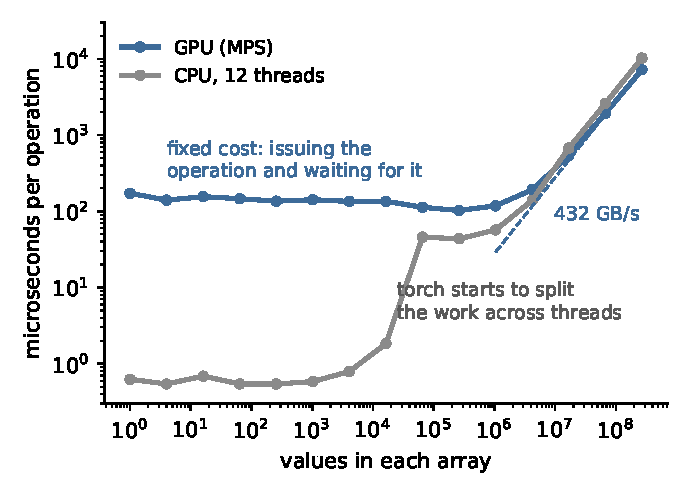
\includegraphics[width=\linewidth]{operation_size.pdf}\\[2pt]
      \figcaption{The time of \texttt{c = a + b} on the M4 Max, with a wait for
      the device after each operation.  The CPU's step near 32 thousand values
      is where torch starts to split an operation across threads.}
    \end{column}
  \end{columns}
  \source{\texttt{demos/demo\_sizes.py} and \texttt{demos/demo\_machine.py};
  \texttt{mbirtorch/projectors.py}}
\end{frame}

% ---------------------------------------------------------------- levels
\begin{frame}{Four levels of control over the hardware}
  \vspace{0pt}
  {\footnotesize
  \begin{tabular}{@{}>{\raggedright\arraybackslash}p{0.13\linewidth}@{\hspace{6pt}}>{\raggedright\arraybackslash}p{0.25\linewidth}@{\hspace{6pt}}>{\raggedright\arraybackslash}p{0.31\linewidth}@{\hspace{6pt}}>{\raggedright\arraybackslash}p{0.25\linewidth}@{}}
    \speclabel{level} & \speclabel{what you write} & \speclabel{what it removes} & \speclabel{what it costs} \rowrule
    \head{Eager torch} & ordinary torch operations & nothing.  Each operation is one kernel that reads and writes memory. & nothing \rowrule
    \head{torch.compile} & the same code, passed to \texttt{torch.compile} & extra trips through memory, by fusing operations.  CUDA graphs also remove most launch costs. & a compile on the first call, and when shapes change \rowrule
    \head{Triton} & a kernel in a Python-like language, one block of values at a time & whatever you choose: which values each block loads and keeps on the chip & a kernel to write and check, for NVIDIA and AMD GPUs \rowrule
    \head{CUDA C++} & a kernel in C++, thread by thread & everything the hardware allows & the most code, for NVIDIA GPUs \\
  \end{tabular}}\par\vspace{8pt}
  \noteline{\texttt{torch.compile} writes Triton kernels for a CUDA GPU and C++
  for a CPU.  It also works on MPS, where Triton and CUDA do not run.}
\end{frame}

% ---------------------------------------------------------------- fusion
\begin{frame}{Fusion reduces the trips through memory}
  \begin{columns}[T]
    \begin{column}{0.50\textwidth}
      {\small
      The qGGMRF surrogate weight in \texttt{mbirtorch/qggmrf.py} is a chain of
      12 elementwise operations.  Eager mode runs 12 kernels, each reading and
      writing full arrays.  \texttt{torch.compile} fuses them into one
      kernel.\par\vspace{5pt}
      {\footnotesize
      \begin{tabular}{@{}l@{\hspace{10pt}}r@{\hspace{10pt}}r@{\hspace{10pt}}r@{}}
        \speclabel{$2^{26}$ values} & \speclabel{eager} & \speclabel{compiled} & \speclabel{speedup} \\[2pt]
        M4 Max GPU (MPS) & 15.8 ms & 1.42 ms & 11.1 \\
        M4 Max CPU & 96.8 ms & 38.2 ms & 2.5 \\
      \end{tabular}}\par\vspace{5pt}
      On the GPU the eager chain is bandwidth-bound, so fusion gains 11 times.
      On the CPU the chain is partly compute-bound, so it gains
      less.\par\vspace{5pt}
      The first compiled call took 9.9 s on the CPU, because it includes the
      compilation.\par}
    \end{column}
    \begin{column}{0.48\textwidth}
      \centering
      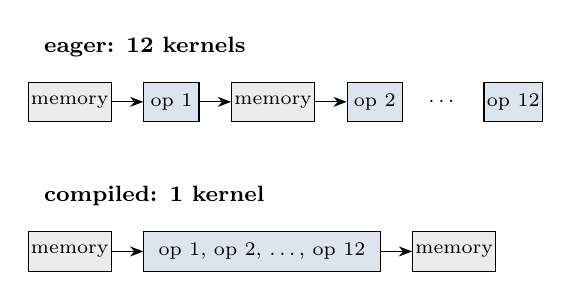
\begin{tikzpicture}[font=\scriptsize, >=Stealth,
          mem/.style={draw, fill=gray!15, minimum width=9mm, minimum height=5mm, inner sep=1pt},
          op/.style={draw, fill=planAccent!18, minimum width=7mm, minimum height=5mm, inner sep=1pt}]
        \node[anchor=west, font=\footnotesize\bfseries] at (0,3.3) {eager: 12 kernels};
        \node[mem] (m0) at (0.45,2.6) {memory};
        \node[op, right=4mm of m0] (o1) {op 1};
        \node[mem, right=4mm of o1] (m1) {memory};
        \node[op, right=4mm of m1] (o2) {op 2};
        \node[right=2mm of o2] (dots) {\dots};
        \node[op, right=2mm of dots] (o12) {op 12};
        \draw[->] (m0) -- (o1); \draw[->] (o1) -- (m1); \draw[->] (m1) -- (o2);
        \node[anchor=west, font=\footnotesize\bfseries] at (0,1.4) {compiled: 1 kernel};
        \node[mem] (n0) at (0.45,0.7) {memory};
        \node[op, minimum width=30mm, right=4mm of n0] (f) {op 1, op 2, \dots, op 12};
        \node[mem, right=4mm of f] (n1) {memory};
        \draw[->] (n0) -- (f); \draw[->] (f) -- (n1);
      \end{tikzpicture}\\[6pt]
      \figcaption{In eager mode every intermediate result goes to memory and
      comes back.  The fused kernel keeps the intermediate results on the
      chip.  The eager and compiled results agree to 3e-7, relative.}
    \end{column}
  \end{columns}
  \source{\texttt{demos/demo\_fusion.py}; \texttt{mbirtorch/qggmrf.py}}
\end{frame}

% ---------------------------------------------------------------- mbirtorch levels
\begin{frame}{How mbirtorch uses the levels}
  \begin{columns}[T]
    \begin{column}{0.48\textwidth}
      {\small
      mbirtorch uses three of the four levels.\par\vspace{5pt}
      \head{Compiled torch code.}  The projectors are torch operations on a
      batch of views, fused by \texttt{torch.compile}.  This path runs on every
      device.\par\vspace{5pt}
      \head{Triton kernels.}  Hand-written kernels replace it for the
      cone-beam, parallel-beam, and multi-axis projectors on CUDA
      GPUs.\par\vspace{5pt}
      \head{A check before use.}  At the first use, each kernel is compared
      with its torch code on a tiny problem, on the device that will run it.
      If the two differ by more than 1e-4, the torch code runs
      instead.\par}
    \end{column}
    \begin{column}{0.50\textwidth}
      {\footnotesize \head{The multi-axis model}, a scan of 1024 views by 1008
      rows by 992 channels, three iterations, after the first call:}\par\vspace{4pt}
      {\footnotesize
      \begin{tabular}{@{}l@{\hspace{5pt}}r@{\hspace{7pt}}r@{\hspace{5pt}}r@{\hspace{5pt}}r@{}}
        & \speclabel{torch code} & \multicolumn{3}{l}{\speclabel{triton kernels}} \\
        & \speclabel{1 gpu} & \speclabel{1 gpu} & \speclabel{2 gpus} & \speclabel{4 gpus} \\[2pt]
        time & 309.9 s & 67.6 s & 37.4 s & 22.8 s \\
        memory & 34.8 GB & 24.1 GB & 13.0 GB & 7.5 GB \\
      \end{tabular}}\par\vspace{4pt}
      \figcaption{H100 GPUs.  Memory is the peak of arrays in use on the
      busiest GPU.  On one GPU the kernels were 4.6 times faster than the
      compiled torch code.  They also used less memory, because they need no
      large temporary arrays.}
    \end{column}
  \end{columns}
  \source{\texttt{mbirtorch/kernel\_availability.py}; \texttt{mbirtorch/projectors.py};
  \texttt{archive/torch\_port/active/multigpu\_findings.md}, Sections 1.45 and 1.46}
\end{frame}

% ================================================================ 5 SEVERAL DEVICES
\section{Several devices}

% ---------------------------------------------------------------- three patterns
\begin{frame}{The first question: must the devices exchange data during a step?}
  \centering
  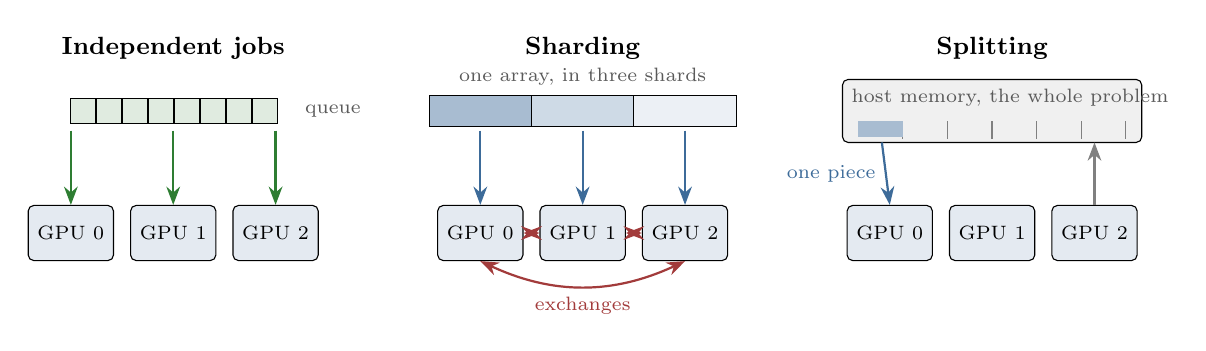
\begin{tikzpicture}[font=\scriptsize, >=Stealth,
      dev/.style={draw, rounded corners=2pt, fill=planAccent!14, minimum width=10mm, minimum height=7mm},
      job/.style={draw, fill=safeGreen!15, minimum width=3.2mm, minimum height=3.2mm, inner sep=0pt},
      host/.style={draw, rounded corners=2pt, fill=gray!12}]
    % ---- independent jobs
    \node[font=\small\bfseries] at (2.0,3.55) {Independent jobs};
    \foreach \k in {0,...,7} { \node[job] at (0.85+0.33*\k,2.75) {}; }
    \node[anchor=west, text=inkGray] at (3.55,2.75) {queue};
    \foreach \i in {0,1,2} {
      \node[dev] (a\i) at (0.7+1.3*\i,1.2) {GPU \i};
      \draw[->, safeGreen, thick] (0.7+1.3*\i,2.5) -- (a\i.north);
    }
    % ---- sharding
    \begin{scope}[xshift=52mm]
      \node[font=\small\bfseries] at (2.0,3.55) {Sharding};
      \foreach \i/\c in {0/planAccent!45, 1/planAccent!25, 2/planAccent!10} {
        \node[draw, fill=\c, minimum width=13mm, minimum height=4mm, inner sep=0pt] at (0.7+1.3*\i,2.75) {};
        \node[dev] (b\i) at (0.7+1.3*\i,1.2) {GPU \i};
        \draw[->, planAccent, thick] (0.7+1.3*\i,2.5) -- (b\i.north);
      }
      \node[anchor=south, text=inkGray] at (2.0,2.95) {one array, in three shards};
      \draw[<->, axialBrick, thick] (b0.east) -- (b1.west);
      \draw[<->, axialBrick, thick] (b1.east) -- (b2.west);
      \draw[<->, axialBrick, thick] (b0.south) to[bend right=25] node[below, text=axialBrick] {exchanges} (b2.south);
    \end{scope}
    % ---- splitting
    \begin{scope}[xshift=104mm]
      \node[font=\small\bfseries] at (2.0,3.55) {Splitting};
      \node[host, minimum width=38mm, minimum height=8mm] (h) at (2.0,2.75) {};
      \node[anchor=north west, text=inkGray] at (h.north west) {host memory, the whole problem};
      \foreach \k in {0,...,5} { \draw[gray] (0.3+0.566*\k+0.566,2.4) -- (0.3+0.566*\k+0.566,2.62); }
      \fill[planAccent!45] (0.3,2.42) rectangle (0.866,2.62);
      \foreach \i in {0,1,2} { \node[dev] (c\i) at (0.7+1.3*\i,1.2) {GPU \i}; }
      \draw[->, planAccent, thick] (0.6,2.35) -- (c0.north) node[midway, left, text=planAccent] {one piece};
      \draw[->, gray, thick] (c2.north) -- (3.3,2.35);
    \end{scope}
  \end{tikzpicture}\par\vspace{4pt}
  {\scriptsize
  \begin{columns}[T]
    \begin{column}{0.31\textwidth}
      Each job fits on one device, and no data moves between devices.  A queue
      hands out the jobs.  Examples: MACE denoising, and a sweep over
      parameters.
    \end{column}
    \begin{column}{0.31\textwidth}
      One problem is split across the devices, and the devices exchange data at
      fixed points.  Examples: an mbirtorch reconstruction on several GPUs, and
      data-parallel training.
    \end{column}
    \begin{column}{0.31\textwidth}
      The problem does not fit on all the devices together.  Pieces are
      processed in turn and assembled in host memory.  Example:
      \texttt{recon\_split\_sino} for a $4096^3$ volume.
    \end{column}
  \end{columns}}\par\vspace{6pt}
  \footnoteline{In SPMD (single program, multiple data), every device runs the
  same program on its own part of the data, as in sharding.  In MPMD, devices
  run different programs, as the MACE agents do.}
\end{frame}

% ---------------------------------------------------------------- queue
\begin{frame}{Independent jobs: one worker per device, fed from a queue}
  \centering
  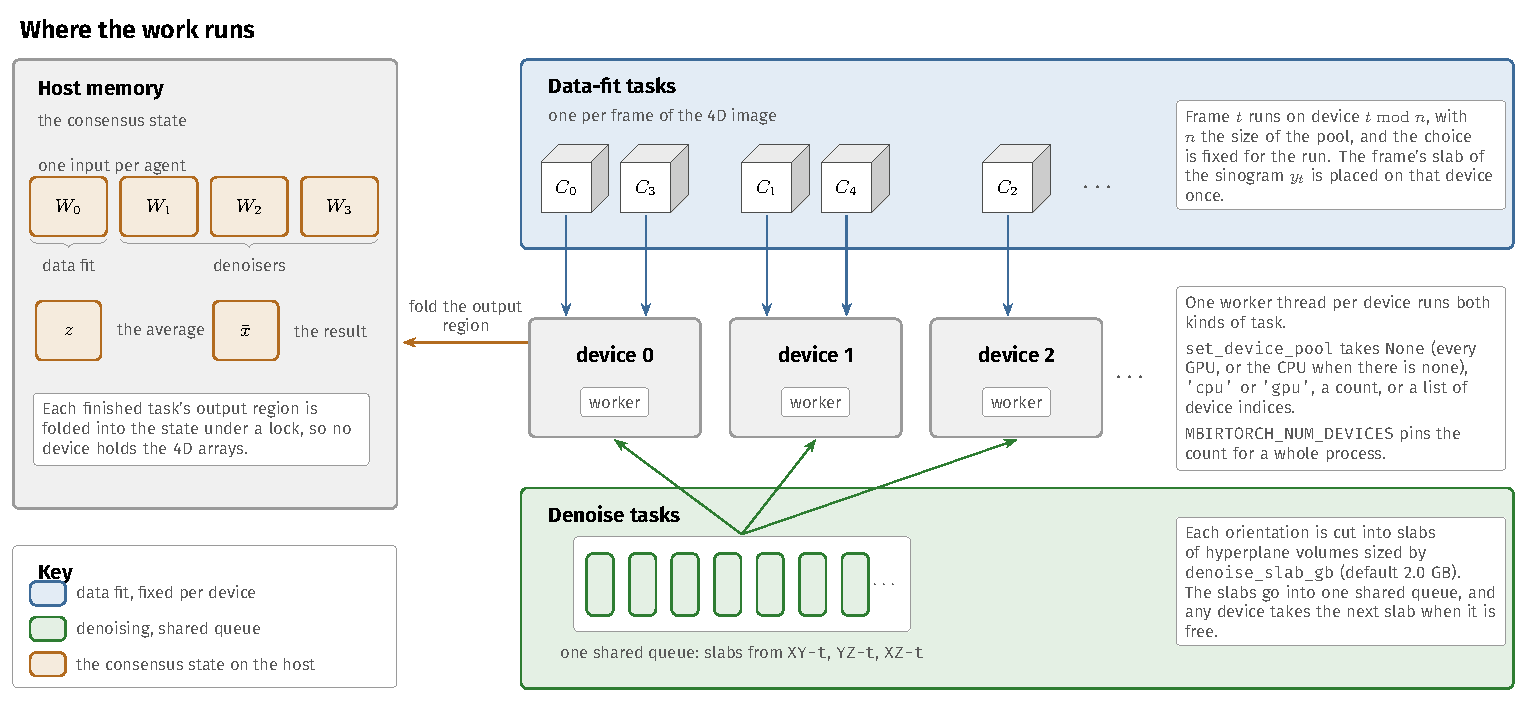
\includegraphics[width=\linewidth,height=0.68\textheight,keepaspectratio]{mace_devices.pdf}\par\vspace{2pt}
  \footnoteline{Each data-fit task stays on the device that holds its frame's
  sinogram.  Denoising tasks wait in one shared queue, and each worker takes
  the next one when it is free.  No data moves between devices.}
  \source{\texttt{mbirtorch/mace.py}; \texttt{plans/mace4d/figures/fig6\_devices.tex}}
\end{frame}

% ---------------------------------------------------------------- sharding
\begin{frame}{Sharding: every device runs the same program on its part}
  \begin{columns}[T]
    \begin{column}{0.50\textwidth}
      {\small
      Every device runs the same program on its shard.  At fixed points the
      devices exchange data through collective operations.\par\vspace{3pt}
      {\footnotesize
      \begin{tabular}{@{}l@{\hspace{8pt}}>{\raggedright\arraybackslash}p{0.64\linewidth}@{}}
        all-reduce & sums over the devices, and gives every device the sum \\
        reduce-scatter & sums, and leaves each device one part of the sum \\
        all-gather & gives every device all of the parts \\
      \end{tabular}}\par\vspace{5pt}
      In JAX the compiler inserts the exchanges from the shardings you
      declare.  In torch, DistributedDataParallel, FSDP, and DTensor insert
      them.\par\vspace{5pt}
      mbirtorch inserts them by hand, with one thread per device.  Back
      projection ends with a reduce-scatter.\par}
    \end{column}
    \begin{column}{0.48\textwidth}
      \centering
      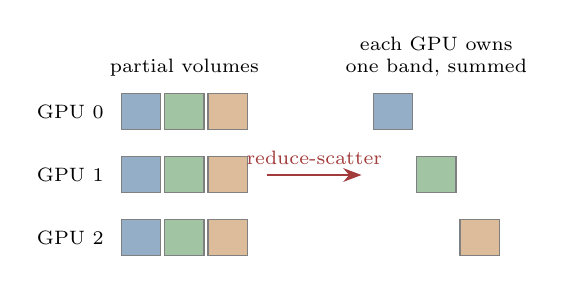
\begin{tikzpicture}[font=\scriptsize, >=Stealth]
        % Left: every GPU holds a partial volume with three bands of slices.
        % Right: after the reduce-scatter, GPU g holds the sum of band g.
        \foreach \g/\c in {0/planAccent!55, 1/safeGreen!45, 2/branchAmber!45} {
          \node[anchor=east] at (-0.1,-0.8*\g+0.22) {GPU \g};
          \foreach \s/\d in {0/planAccent!55, 1/safeGreen!45, 2/branchAmber!45} {
            \filldraw[fill=\d, draw=gray] (0.55*\s, -0.8*\g) rectangle ++(0.5,0.45);
          }
          \filldraw[fill=\c, draw=gray] (3.2+0.55*\g, -0.8*\g) rectangle ++(0.5,0.45);
        }
        \node[anchor=south] at (0.8,0.55) {partial volumes};
        \node[anchor=south, align=center] at (4.0,0.55) {each GPU owns\\one band, summed};
        \draw[->, thick, axialBrick] (1.85,-0.58) -- (3.05,-0.58) node[midway, above, text=axialBrick] {reduce-scatter};
      \end{tikzpicture}\\[6pt]
      \figcaption{Back projection on three GPUs.  Each GPU back-projects its own
      views into a partial volume with three bands of slices.  The
      reduce-scatter sums the partial volumes and leaves each GPU the sum for
      one band.}
    \end{column}
  \end{columns}
  \source{\texttt{mbirtorch/\_sharding.py}}
\end{frame}

% ---------------------------------------------------------------- sharding pays
\begin{frame}{Sharding cuts the memory per GPU, and the time above a crossover size}
  \begin{columns}[T]
    \begin{column}{0.48\textwidth}
      {\small
      Sharding cuts the memory per GPU almost in proportion to the number of
      GPUs.  It cuts the time only when each GPU's share of the work outweighs
      the exchanges.\par\vspace{5pt}
      Below some problem size one GPU is faster, so mbirtorch chooses the GPU
      count from a measured table.  \texttt{MBIRTORCH\_NUM\_DEVICES} fixes the
      count instead.\par\vspace{6pt}}
      \footnoteline{In mbirjax, sharded back projection beat one GPU only with
      3 or more GPUs.}
    \end{column}
    \begin{column}{0.50\textwidth}
      {\footnotesize \head{The multi-axis model with Triton kernels}, a scan
      of 1024 views by 1008 rows by 992 channels, on H100 GPUs:}\par\vspace{4pt}
      {\footnotesize
      \begin{tabular}{@{}l@{\hspace{10pt}}r@{\hspace{10pt}}r@{\hspace{10pt}}r@{}}
        & \speclabel{1 gpu} & \speclabel{2 gpus} & \speclabel{4 gpus} \\[2pt]
        time & 67.6 s & 37.4 s & 22.8 s \\
        memory on the busiest GPU & 24.1 GB & 13.0 GB & 7.5 GB \\[3pt]
        time, relative to 1 GPU & 1 & 0.55 & 0.34 \\
        memory, relative to 1 GPU & 1 & 0.54 & 0.31 \\
      \end{tabular}}\par\vspace{4pt}
      \figcaption{This problem is large, so both the time and the memory fell
      nearly in proportion to the number of GPUs.}
    \end{column}
  \end{columns}
  \source{\texttt{archive/torch\_port/active/multigpu\_findings.md}, Sections 1.45 and 1.46;
  \texttt{.claude/lessons.md}, Section 6}
\end{frame}

% ---------------------------------------------------------------- splitting
\begin{frame}{When all the GPUs together are not enough, split the problem}
  \begin{columns}[T]
    \begin{column}{0.52\textwidth}
      {\small
      Collaborators need a parallel-beam reconstruction from a 4096 by 4096
      detector with 900 views.  The volume is 275 GB in float32.  Even on 8
      GPUs the problem needs 136 GiB per GPU, more than an H100
      holds.\par\vspace{5pt}
      In parallel beam, detector row $r$ sees only slice $r$, so the rows split
      exactly.  \texttt{recon\_split\_sino} reconstructs one band of rows at a
      time and joins the bands in host memory.  On 8 GPUs it needs 3
      parts.\par\vspace{5pt}
      Joining the bands needs about 800 GB of host memory.  A streaming script
      writes each band to disk instead, and needs about 90 GB.\par}
    \end{column}
    \begin{column}{0.46\textwidth}
      {\footnotesize \head{Modeled peak on the busiest GPU}, GiB:}\par\vspace{4pt}
      {\footnotesize
      \begin{tabular}{@{}r@{\hspace{8pt}}r@{\hspace{10pt}}r@{\hspace{8pt}}r@{\hspace{8pt}}r@{\hspace{8pt}}r@{}}
        \speclabel{parts} & \speclabel{slices} & \speclabel{1 gpu} & \speclabel{2 gpus} & \speclabel{4 gpus} & \speclabel{8 gpus} \\[2pt]
        1 & 4096 & 1078 & 540 & 270 & 136 \\
        2 & 2053 & 541 & 271 & 136 & 69 \\
        3 & 1376 & 363 & 182 & 92 & \textbf{46.5} \\
        4 & 1034 & 273 & 137 & 69 & 35 \\
        8 & 522 & 139 & 70 & 36 & 20 \\
        16 & 266 & 71 & 36 & 20 & 13 \\
      \end{tabular}}\par\vspace{4pt}
      \figcaption{A part fits when 1.15 times its peak is at most the free
      memory of the card, about 80 GB on an H100.  Each seam between parts has
      5 rows of overlap for the prior.}
    \end{column}
  \end{columns}
  \source{\texttt{plans/parallel\_4k/plan.md}}
\end{frame}

% ================================================================ 6 MEMORY
\section{Memory}

% ---------------------------------------------------------------- where memory goes
\begin{frame}{Where GPU memory goes}
  \begin{columns}[T]
    \begin{column}{0.50\textwidth}
      {\small
      One GPU's memory has four levels: the arrays held for the whole run,
      the peak of arrays in use, the memory reserved by torch's caching
      allocator, and the \texttt{nvidia-smi} total, which adds the CUDA
      context.  On the busiest H100 of the ORNL scan these were 15.3, 29.0,
      38.4, and 39.7 GiB.\par\vspace{5pt}
      The peak came from one setup step that held five sinogram-sized arrays.
      Temporary arrays, not the data, set the peak.\par\vspace{6pt}}
      \footnoteline{\texttt{torch.cuda.max\_memory\_allocated()} and
      \texttt{torch.cuda.memory\_reserved()} read the second and third
      levels.}
    \end{column}
    \begin{column}{0.48\textwidth}
      \centering
      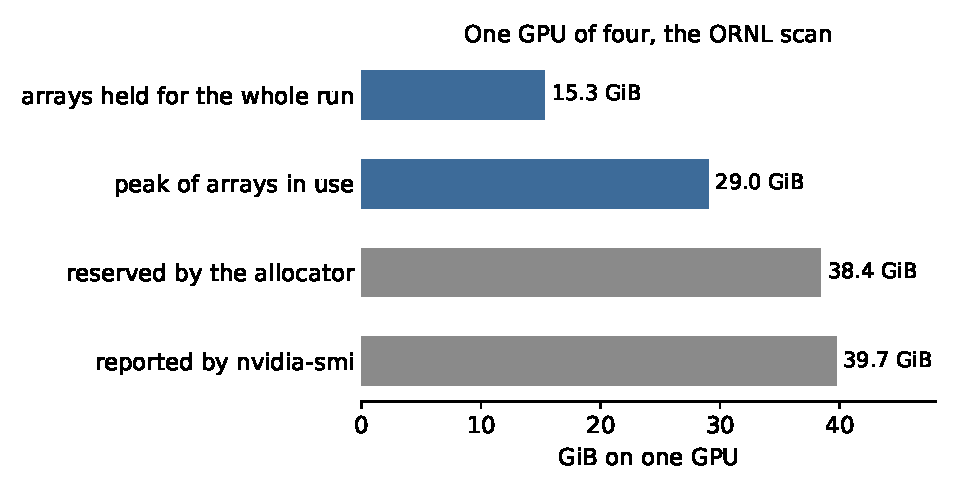
\includegraphics[width=\linewidth]{memory_levels.pdf}\\[2pt]
      \figcaption{The ORNL Inconel scan, 2132 views by 1456 by 1840, on four
      H100 GPUs, 15 iterations, before the memory changes of September
      2026.}
    \end{column}
  \end{columns}
  \source{\texttt{surveys/leap\_comparison/findings/ornl\_reproduction.md}, Sections 3.1 and 3.2;
  \texttt{plans/device\_memory\_tiers/plan.md}}
\end{frame}

% ---------------------------------------------------------------- copies
\begin{frame}{Copies: move data once, in large pieces, from pinned memory}
  \begin{columns}[T]
    \begin{column}{0.50\textwidth}
      {\small
      PCIe carries at most 64 GB/s, about 1/50 of the rate of the H100's own
      memory.  Three rules follow.\par\vspace{2pt}
      \begin{enumerate}
        \item Move data to the GPU once, and keep it there.
        \item Copy from pinned host memory, which the GPU reads directly.
        \item Issue copies on a separate stream, so that they overlap with
          arithmetic.
      \end{enumerate}\vspace{3pt}
      \head{An example.}  Gathering a reconstruction from four H100s into one
      8.9 GiB host array took 5.7 s, one GPU at a time on one thread.
      Copying from all GPUs at once, in 16 MiB pieces through pinned memory,
      takes 0.24 s.\par}
    \end{column}
    \begin{column}{0.48\textwidth}
      \centering
      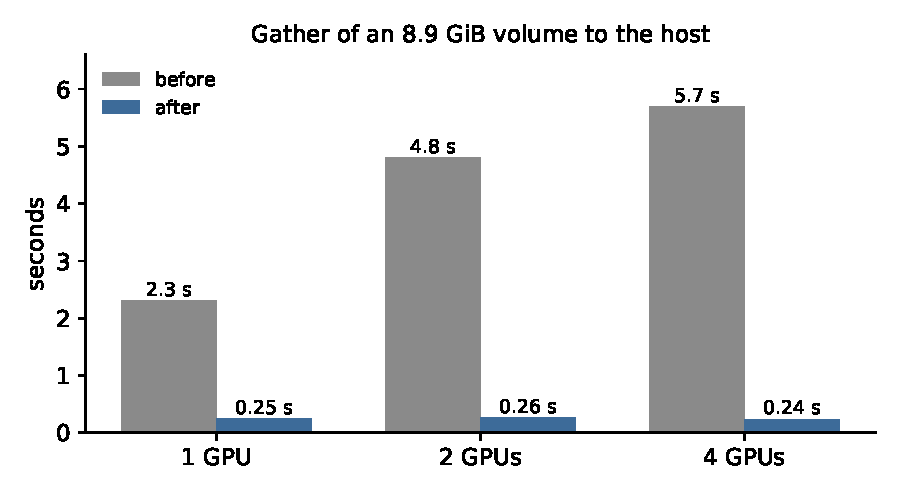
\includegraphics[width=\linewidth]{gather_time.pdf}\\[2pt]
      \figcaption{The time to gather a sharded 8.9 GiB volume into host memory
      on gautschi H100 nodes, before and after the change.}
    \end{column}
  \end{columns}
  \source{\texttt{surveys/leap\_comparison/findings/host\_gather.md}; \texttt{mbirtorch/\_sharding.py}}
\end{frame}

% ---------------------------------------------------------------- trades
\begin{frame}{Memory and time trade against each other}
  \vspace{0pt}
  {\small Each choice below trades memory for time.}\par\vspace{6pt}
  {\footnotesize
  \begin{tabular}{@{}>{\raggedright\arraybackslash}p{0.17\linewidth}@{\hspace{8pt}}>{\raggedright\arraybackslash}p{0.37\linewidth}@{\hspace{8pt}}>{\raggedright\arraybackslash}p{0.37\linewidth}@{}}
    \speclabel{choice} & \speclabel{more memory, less time} & \speclabel{less memory, more time} \rowrule
    batch size & a large \texttt{view\_batch\_size}, with large temporary arrays & a small \texttt{view\_batch\_size} \rowrule
    system matrix & store the matrix and reuse it, as svmbir does & recompute each projection when it is needed, as mbirjax and mbirtorch do \rowrule
    where arrays live & in GPU memory for the whole run & in host memory, with pieces streamed to the GPUs \rowrule
    intermediate results & keep them for reuse & recompute them when they are needed \\
  \end{tabular}}\par\vspace{10pt}
  \noteline{A smaller number type saves both memory and time.  float32 has half
  the bytes of float64, so bandwidth-bound work runs about twice as fast.  MPS
  has no float64.  Tensor-core formats such as TF32 and bfloat16 go further, at
  lower precision.}
\end{frame}

% ================================================================ 7 MEASURING
\section{Measuring honestly}

% ---------------------------------------------------------------- rules
\begin{frame}[fragile]{Rules for timing and memory measurements}
  \begin{columns}[T]
    \begin{column}{0.50\textwidth}
      {\small
      \begin{enumerate}
        \item Synchronize the device before each reading of the clock.
        \item Time the first call separately, because it includes compiling
          and allocation.
        \item Keep the inputs on the device, so that the timing excludes
          copies.
        \item Report the median of several calls.
        \item Reset the peak-memory counter for each configuration.
        \item Record the GPU model, SXM or PCIe, its clock, and its
          temperature.
        \item Check a small benchmark's speedup against the whole program.
      \end{enumerate}}
    \end{column}
    \begin{column}{0.48\textwidth}
      {\small The timing function of the demos, from \texttt{demos/devtime.py}:}
      \begin{lstlisting}
def time_call(fn, device, repeats=10, warmup=2):
    for _ in range(warmup):
        fn()
    times = []
    for _ in range(repeats):
        synchronize(device)
        start = time.perf_counter()
        fn()
        synchronize(device)
        times.append(time.perf_counter() - start)
    return statistics.median(times)
      \end{lstlisting}
    \end{column}
  \end{columns}
  \source{\texttt{.claude/lessons.md}, Section 5; \texttt{demos/devtime.py}}
\end{frame}

% ---------------------------------------------------------------- stories
\begin{frame}{Five measurements that misled us}
  \vspace{0pt}
  {\footnotesize
  \begin{tabular}{@{}>{\raggedright\arraybackslash}p{0.30\linewidth}@{\hspace{10pt}}>{\raggedright\arraybackslash}p{0.64\linewidth}@{}}
    \speclabel{what we saw} & \speclabel{what was really measured} \rowrule
    An M3 Mac looked faster than an H100 node. & The JAX benchmark built its jit inside the timed call, so every call traced the function again.  The tracing turned a 1 ms step into 1,828 ms. \rowrule
    A kernel looked 1.45 times faster than the old code. & The inputs came from host memory, so the timing included a copy.  With the inputs already on the GPU, the kernel was 2.25 times faster. \rowrule
    A code change looked like a slowdown. & One H100 was throttling: it was hot and its clock was low.  The slowdown appeared only at large sizes, and only when that card was in use. \rowrule
    Wall times from one partition did not agree. & gilbreth's \texttt{a100-40gb} partition mixes A100 SXM4 nodes and A100 PCIe nodes, whose clocks differ.  A timing job must request one kind with \texttt{-{}-constraint}. \rowrule
    A kernel 2.13 times faster in isolation made the library slower, 0.68 times as fast. & The library copied a value to the host for every chunk of views, and it sized each launch from the data, so each new subset forced a recompile.  After the fix the library was 2.57 times faster. \\
  \end{tabular}}
  \source{\texttt{.claude/lessons.md}, Section 5; \texttt{.claude/cluster\_use.md}}
\end{frame}

% ================================================================ summary
\section{Summary}

\begin{frame}{Summary}
  \medskip
  {\small
  \begin{enumerate}
    \item Know where your data is.  The links between memories and processors
      differ in speed by a factor of 50 or more.\vspace{1pt}
    \item Find the limit that applies: overhead, memory bandwidth, compute, or
      capacity.  Arithmetic intensity separates bandwidth from
      compute.\vspace{1pt}
    \item A GPU call returns before its work is done.  Synchronize before
      reading the clock, and avoid host waits inside loops.\vspace{1pt}
    \item Use one device fully before using several.  Batch the work, then
      compile it, then write kernels where the gain justifies the
      effort.\vspace{1pt}
    \item Choose the pattern for several devices by what they must exchange.
      Use a queue for independent jobs, sharding for a problem too large for
      one device, and splitting for a problem too large for all of
      them.\vspace{1pt}
    \item Temporary arrays set the peak memory.  Measure it.\vspace{1pt}
    \item Check every speedup against the whole program.
  \end{enumerate}}
\end{frame}

% ================================================================ BACKUP
\appendix

% A standout frame instead of \section: the theme's section page fails in the
% appendix when appendixnumberbeamer resets the frame count.
\begin{frame}[standout]
  Backup slides
\end{frame}

% ---------------------------------------------------------------- vocabulary
\begin{frame}{The same ideas in JAX and torch}
  \vspace{0pt}
  {\footnotesize
  \begin{tabular}{@{}>{\raggedright\arraybackslash}p{0.30\linewidth}@{\hspace{8pt}}>{\raggedright\arraybackslash}p{0.30\linewidth}@{\hspace{8pt}}>{\raggedright\arraybackslash}p{0.33\linewidth}@{}}
    \speclabel{idea} & \speclabel{jax} & \speclabel{torch} \rowrule
    batch a function & \texttt{jax.vmap} & \texttt{torch.vmap} \rowrule
    compile and fuse & \texttt{jax.jit} & \texttt{torch.compile} \rowrule
    place an array on a device & \texttt{jax.device\_put(x, device)} & \texttt{x.to('cuda:1')} \rowrule
    shard an array, with the exchanges inserted for you & \texttt{jax.jit} with a \texttt{Mesh} and \texttt{NamedSharding} & DTensor \rowrule
    per-device code with explicit exchanges & \texttt{shard\_map} & \texttt{torch.distributed} collectives, or one thread per device as in mbirtorch \rowrule
    one process per device & \texttt{jax.distributed.initialize} & \texttt{torchrun} with DistributedDataParallel or FSDP \rowrule
    collective operations & \texttt{psum}, \texttt{all\_gather}, \texttt{psum\_scatter} & \texttt{all\_reduce}, \texttt{all\_gather}, \texttt{reduce\_scatter} \rowrule
    older interfaces & \texttt{jax.pmap} & \texttt{torch.nn.DataParallel} \\
  \end{tabular}}
\end{frame}

% ---------------------------------------------------------------- gautschi
\begin{frame}[fragile]{Getting GPUs on gautschi}
  \begin{columns}[T]
    \begin{column}{0.46\textwidth}
      {\small A batch header for one H100:}
      \begin{lstlisting}[language=bash]
#SBATCH -A bouman
#SBATCH -p ai
#SBATCH -N 1
#SBATCH --gpus-per-node=1
#SBATCH --cpus-per-task=14
#SBATCH -t 04:00:00
      \end{lstlisting}\vspace{4pt}
      {\small To see what the job received:}
      \begin{lstlisting}[language=bash]
nvidia-smi            # GPUs, memory, clocks
nvidia-smi topo -m    # the links between GPUs
nproc                 # CPU cores for this job
      \end{lstlisting}
    \end{column}
    \begin{column}{0.52\textwidth}
      {\small
      \begin{itemize}
        \item The \texttt{ai} partition requires 14 CPUs for each GPU, and it
          refuses \texttt{-{}-mem}.  Host memory is fixed at about 126 GB per
          GPU, so more host memory means more GPUs.
        \item A job without \texttt{-t} gets 30 minutes.
        \item GPU-hours are metered, and \texttt{slist} shows the group's
          balance.  An idle allocation uses GPU-hours at the full rate, so
          release it when you are done.
        \item On gilbreth, a timing job on the \texttt{a100-40gb} partition
          needs \texttt{-{}-constraint=N} (SXM4) or \texttt{-{}-constraint=G}
          (PCIe).
      \end{itemize}}
    \end{column}
  \end{columns}
  \source{\texttt{.claude/cluster\_use.md}}
\end{frame}

% ---------------------------------------------------------------- 2^31
\begin{frame}{Very large arrays: the \texorpdfstring{$2^{31}$}{2\textasciicircum 31} boundary}
  \vspace{0pt}
  {\small
  A full-size sinogram or reconstruction can hold 4.6 to 4.8 billion
  elements.  That is more than $2^{31} \approx 2.1$ billion, the largest value
  a signed 32-bit integer holds.  Several mechanisms fail there, most of them
  without an error, and small test problems never reach the
  boundary.\par\vspace{6pt}
  \begin{itemize}
    \item An index stored as int32 wraps.  In JAX, \texttt{argmin} over more
      than $2^{31}$ elements returned an index off by exactly $2^{32}$.
    \item In JAX, a Python int larger than $2^{31}$ passed into jitted code
      raises an OverflowError.  Pass element counts as floats, or as static
      arguments.
    \item \texttt{np.prod} of a shape uses the platform's default integer,
      which is int32 on Windows with NumPy before 2.0.  Use \texttt{math.prod}
      for element counts.
    \item A float32 count stops growing at $2^{24}$, because adding 1 no
      longer changes it.  Count in int64, or in slabs of fewer than $2^{31}$.
  \end{itemize}}
  \source{\texttt{.claude/lessons.md}, Section 4}
\end{frame}

% ---------------------------------------------------------------- precision
\begin{frame}{Precision on each device}
  \vspace{0pt}
  {\footnotesize
  \begin{tabular}{@{}>{\raggedright\arraybackslash}p{0.16\linewidth}@{\hspace{8pt}}>{\raggedright\arraybackslash}p{0.76\linewidth}@{}}
    \speclabel{device} & \speclabel{what to expect} \rowrule
    CPU & float64 is fully supported.  Vectorized float64 arithmetic runs at about half the float32 rate, because each vector holds half as many values. \rowrule
    H100 & float64 runs at 34 TFLOP/s, half of float32's 67 TFLOP/s without tensor cores.  With tensor cores, TF32 matrix products reach about 495 TFLOP/s. \rowrule
    MPS & There is no float64.  A float64 tensor cannot be moved to \texttt{'mps'}. \rowrule
    torch & torch uses TF32 for float32 matrix products on a CUDA GPU only when asked, with \texttt{torch.set\_float32\_matmul\_precision('high')}. \\
  \end{tabular}}\par\vspace{10pt}
  \noteline{For bandwidth-bound work, the number of bytes sets the time.  Halving
  the bytes per value halves the time, whatever the arithmetic rate.}
  \source{NVIDIA H100 SXM specification; the torch documentation}
\end{frame}

% ---------------------------------------------------------------- M4 Max numbers
\begin{frame}{The measured numbers for the M4 Max}
  \begin{columns}[T]
    \begin{column}{0.48\textwidth}
      {\footnotesize \head{demo\_machine.py}}\par\vspace{3pt}
      {\footnotesize
      \begin{tabular}{@{}l@{\hspace{10pt}}r@{\hspace{10pt}}r@{}}
        & \speclabel{cpu} & \speclabel{gpu (mps)} \\[2pt]
        matrix product, TFLOP/s & 3.03 & 13.40 \\
        bandwidth of \texttt{c = a + b}, GB/s & 316 & 432 \\
        one small operation, microseconds & 1.1 & 3.3 \\
        copy host to GPU, GB/s & & 89 \\
        copy GPU to host, GB/s & & 44 \\
      \end{tabular}}\par\vspace{8pt}
      {\footnotesize \head{demo\_async.py}, an 8192 by 8192 product on MPS}\par\vspace{3pt}
      {\footnotesize
      \begin{tabular}{@{}l@{\hspace{10pt}}r@{}}
        the call returned & 0.11 ms \\
        \texttt{synchronize()} returned & 81.9 ms \\
        \texttt{.item()} returned & 82.0 ms \\
      \end{tabular}}
    \end{column}
    \begin{column}{0.50\textwidth}
      {\footnotesize \head{demo\_fusion.py}, the qGGMRF weight on $2^{26}$ values}\par\vspace{3pt}
      {\footnotesize
      \begin{tabular}{@{}l@{\hspace{8pt}}r@{\hspace{8pt}}r@{\hspace{8pt}}r@{}}
        & \speclabel{eager} & \speclabel{compiled} & \speclabel{first call} \\[2pt]
        CPU & 96.8 ms & 38.2 ms & 9.9 s \\
        GPU (MPS) & 15.8 ms & 1.42 ms & 0.12 s \\
      \end{tabular}}\par\vspace{8pt}
      \figcaption{The CPU matrix product runs in Apple's Accelerate library.
      The small-operation cost is measured without a wait after each
      operation.  The MPS first compiled call ran after the CPU compile in the
      same process.  Repeated runs of the thread demo varied by up to 15
      percent.  torch 2.14.0, September 24, 2026.}
    \end{column}
  \end{columns}
  \source{\texttt{demos/results/}}
\end{frame}

\end{document}
